\documentclass[12pt,journal,draftclsnofoot,onecolumn]{IEEEtran}
%\documentclass[12pt,journal]{IEEEtran}
\IEEEoverridecommandlockouts
\usepackage{cite}  
\usepackage{amsmath,amssymb,amsfonts}
\usepackage{algorithm}
\usepackage{algorithmic} 
\usepackage{textcomp}
\usepackage{xcolor}    
\usepackage{amsthm}  
\usepackage{graphicx}
\usepackage{multirow}  
%\usepackage{algpseudocode}
\usepackage{booktabs}
 
\renewcommand{\algorithmicrequire}{\textbf{Input:}} 
\renewcommand{\algorithmicensure}{\textbf{Output:}} 
 
\def\BibTeX{{\rm B\kern-.05em{\sc i\kern-.025em b}\kern-.08em
		T\kern-.1667em\lower.7ex\hbox{E}\kern-.125emX}}

 %just trying something
%\geometry{left=2.54cm,right=2.54cm,top=1.0cm,bottom=1.0cm}

%Iyemeh: The title should show that this is an approach, method or strategy. I have included strategy in the heading as this was used a lot in the paper. 

\title{Joint Path Planning and Power Allocation Strategy for Multitarget Tracking in Multistatic Radar System}
\author{Anbang Deng, Thiagalingam Kirubarajan, Ratnasingham Tharmarasa}
\date{}
\begin{document}
\maketitle

\begin{abstract}
% Multistatic radar systems have prominent advantages over traditional monostatic radar systems in practicabilities and potential tracking capabilities.
Multistatic radar systems have the advantage of practiacabilities and potential tracking capabilities over traditional monostatic radar systems.
%Iyemeh: The practicabilities is vague and should be quantified, eg. easier to implement or more realistic or efficient. Also the potential tracking capabilities should also be explained. 
% An effective utilization of limited power and a proper deployment of sensors can significantly improve the performance of the system. 
%Iyemeh: The sentence above sounds like it is standing alone, no connection with the previous sentence. I have rephrased below:
Multistatic radar systems can be improved by optimizing limited power and efficient deployment of sensors for multitarget tracking applications. 
This paper presents a joint path planning and power allocation (JPPPA) strategy for tracking multiple targets in a multistatic radar system having a fixed transmitter and multiple moving receivers. 
%The allocation scheme for transmitted power and the paths of receivers are jointly optimized and controlled so that the system may obtain more accurate state estimation. 
%Iyemeh: I have revised the sentence above, however, I think the term state is vague and should be ellaborate. Is the state the position, or speed, what exactly is the state?
This approach optimizes and controls the allocation scheme of transmitted power and the paths of receivers to obtain accurate speed and heading angle estimation.
%The Posterior Cramér-Rao lower bound (PCRLB) gives a measure of the optimal achievable performance of an unbiased estimator, and is thus derived and utilized as a criterion for the resource management strategy. 
To measure the optimal performance of an unbiased estimating approach, the Posterior Cramer-Ratio Lower Bound (PCRLB) is derived and used as the basis for the resource management strategy. %Iyemeh: Strategy does not sound right in this place. 
%Iyemeh: This sentence "It is shown that the JPPPA optimizaiton is a three-variable nonconvex problem." can be deleted without losing anything. As it stands, the three variables needed for the JPPPA optimization will need to be stated to add significant details to the abstract.  
A modified genetic algorithm (GA) with a custom pre-selection operator is developed to determine the power allocation scheme and sensor movement simultaneously. A receding horizon control (RHC) framework is applied to offer fault tolerance and provide the system with long-term guidance. The proposed algorithm is compared to a two-step algorithm which incorporates dynamic programming for path planning. Results show that the tracking performance in terms of estimation accuracy can be improved by the JPPPA strategy. The effectiveness of the proposed pre-selection operator is verified through comparison with ordinary genetic algorithm. Results show that the pre-selection operator makes use of the extra information from the RHC sequence and accelerates the convergence of GA.

    
\end{abstract}

\begin{IEEEkeywords}
Multitarget tracking, resource management, path planning, power allocation multistatic radar, Posterior Cramér-Rao lower bound
\end{IEEEkeywords}


\section{Introduction}
\subsection{Background and Motivation}
Multistatic radar systems have attracted considerable interests in recent years. Characterized by the separation between transmitters and receivers, multistatic radars provide the capability to handle more difficult tasks, %Iyemeh: The more difficult tasks should be listed. Leaving it as more difficult tasks is vague. 
 especially in dangerous or hostile environments. %Whether by utilizing illuminators of oppoturnity, with the receivers being passive, or by working cooperatively with numbers of transmitters and receivers, multistatic radars have shown to offer significant adavantages over traditional monostatic radars in civil and military applications such as area surveillance and environmental monitoring. %Iyemeh: The sentence is rephrased below
Multistatic radars offer significant advantages over traditional monostatic radars in civil and military applications in applications such as surveillance and environmental monitoring by utilizing illuminators of opportunity with passive receivers and working cooperatively with several transmitters and receivers\cite{handel1986survey}. %While more potentials of multistatic radars are being exploited, the resource management problems in such systems arise in order to satisfy technical requirements such as better tracking performance or more reasonable resource allocation. 
With the discovery of new applications for multistatic radars, there is a rising challenge in the system's resource management which ensures that better tracking performance and adequate resource allocation are met. The configuration of resources in radar systems has a an effect on the capability of trackers, especially in multistatic radars where tracking accuracy is affected by the bistatic geometry and a small change in the receivers' position may bring significant improvement.

 The aim of resource management, in the field of target tracking, is to achieve accurate state estimation by properly deploying limited resources, or to lower the the estimation errors to a certain threshold\cite{hero2011sensor}. Originally, resource management only concerns the deployment of sensors, and thus is commonly referred to as sensor management. Based on the configuration of sensors, the main problems of sensor management include optimal sensor selection\cite{tharmarasa2011decentralized,zhan2010adaptive,tharmarasa2009optimization}, optimal sensor placement\cite{xu2017optimal,nguyen2016optimal} and path planning of mobile sensors\cite{tharmarasa2009joint,he2019trajectory,huang2007static,scott2018illuminator}. The objective of sensor management is to determine the behaviors of sensors, such as the trajectories of movable sensors, to optimize the tracking performance subject to their operational constrains. Sensor management has been studied for decades, considerable concepts and algorithms have been addressed in the literature\cite{tharmarasa2007pcrlb,tharmarasa2011decentralized,hernandez2004multisensor,dogancay2007online,douganccay2010single}. Recently, other resources, such as power or communication channels, are incorporated into sensor management, making them more practical in real-life scenarios.

%Unmaned aerial vehicles (UAVs) have been considerably studied in the literature and widely employed in real-life applications\cite{pitre2012uav}. These small and affordable devices are proper platforms to mount receivers in a multistatic radar system. %Iyemeh: The first sentence in this paragraph seems disjointed from the rest of the text. Hence, it is proper to discuss the UAV from the perspective of Multistatic radar systems. I have revised below.
Multistatic radar systems could integrate the use of receivers mounted on small and affordable Unmanned Aerial Vehicle (UAVs). UAVs have been well studied in literature and widely employed in real-life applications\cite{pitre2012uav}. Studies on UAV's path planning have provided fundamental background for sensor management problems in multistatic radar systems. % Sensor management, e.g., path planning or sensor deployment, plays a vital role in radar systems. An ideal position of sensors will contribute significantly to a better tracking performance. %Iyemeh: This has been stated earlier and should be deleted.
  The positions or trajectories of sensor are important in multistatic radars due to the complicated transmitter-target-receiver triangle.

In \cite{hernandez2004optimal}, an optimal path planning problem using bearing-only measurement is presented and a searching technique is developed. This work provides a basic framwork for the path planning problem in multistatic radar systems. In \cite{dogancay2012uav}, a nonlinear programming problem that maximizes the determinant of the Fischer Information Matrix (FIM) to minimize localization uncertainty is addressed. Conventional optimization algorithms such as gradient descend are used to solve the formulated path planning problem\cite{bruna2017airborne}.%Iyemeh: what formulated problem? I have added path planning to the sentence, kindly replace if it is not the right one.
 In \cite{ragi2013uav}, the path planning is modeled as a partially observable Markov decision process and solved through NBO %Iyemeh: First mention, kindly define. 
 approximation. Convex relaxation is also studied in some papers\cite{xie2017joint}\cite{yan2016joint}. Heuristic methods such as Genetic Algorithm (GA) and Particle Swarm Optimization (PSO) are presented in \cite{roberge2012comparison}.%Iyemeh: More details needed. These algorithms are studied in relation to what? If possible, how do they perform based on the studies? Some comments on their suitability and flaws with respect to the problem should be mentioned and discussed. 
%Iyemeh: The paragraph above seem to discuss path planning. I have moved it closer to where it should be. Please update the citiations in numerical order. 

Power allocation is another critical problem in resource-aware systems. In a radar system, the transmitters have limited power budgets to generate multiple beams that illuminate different targets. How to properly allocate the power resources determines the integral performance of the radar system. Some UAVs that carry the receivers are equipped with batteries, however the UAVs' trajectories need to be optimized under the constraint of limited power supply.%Iyemeh: The sentence suggest that receivers on some UAVs may not have power issue. Hence, we need to add "however" to balance the sentence.


%Considerable efforts have been dedicated %Iyemeh: We cannot quantify what "considerable efforts". Hence, the sentence should read:
Several authors have focused on the power allocation problem in radar systems\cite{alirezaei2014optimum,lu2018adaptive}. In \cite{yan2016joint}, a joint beam selection and power allocation strategy that minimizes the trace of Posterior Cramer-Rao Lower Bound (PCRLB) is proposed to handle the scenario where the transmitter cannot launch enough beams to track all the targets simultaneously. The noncovex problem is solved by a two-step gradient projection method after variable partitioning. %Iyemeh: This is the first mention of the term nonconvex problem. If it is the scenario presented in the previous sentence, then I suggest it is stated in the that sentence before it is used here. Otherwise, a definition of the nonconvex problem would be proper. Also, there should be a reference to where the nonconvex problem was solved. 
In \cite{xie2017joint}, a similar problem where the selection of fusion nodes was considered in a decentralized radar network. A large number of studies regarding low probability of interception (LPI) address the issue of power allocation\cite{she2016novel}\cite{godrich2011power}.




Although path planning and power allocation are both important issues to address in multistatic radar systems, they are barely considered together %Iyemeh: Why should they be considered together? Hence state or show how they are related for there to be an efficient multistatic radar system. This will highlight the gap in literature and also the novelty of the work.
to the best of our knowledge. More precisely, the criteria used for these two porblems are generally different. Therefore, it is hard to formulate them into an integral problem. A common approach would be the adoption of weighted-sum model where multiple objectives are integrated into one metric with respective user-defined weights. The result of such optimizaiton problem is essentially a Pareto trade-off that depends on how much weight the user gives to each individual problem. Therefore, the result is subjective and thus does not offer adequate guidance to the system. Besides, measurement origin uncertainty (MOU) is often neglected in similar works because it will change the convexity of functions that contain PCRLB, making it hard to use convex optimization techniques to solve the problem, while MOU is a realistic issue that needs to be considered in general situations.

The Posterior Cramér-Rao lower bound (PCRLB), which is defined as the inverse of Fishcer Information Matrix, provides a lower bound of the estimation mean squared error (MSE) for any unbiased estimator. The PCRLB can be calculated in a recursive manner\cite{tichavsky1998posterior}, and it is shown in\cite{niu2012target} that under the assumption that the measurement noise is Gaussian, the estimaion error asymptotically approaches the PCRLB in high SNR. Therefore, PCRLB is a suitable criterion where the tracking performance is the objective to optimize\cite{hernandez2004multisensor,tharmarasa2007pcrlb,punithakumar2006multisensor}. Error covariance is also used in some works\cite{douganccay2010single}. 

In this paper, a multistatic radar system with one fixed transmitter and several movable receivers tracking multiple airborne targets is presented. The transmitter is capable of launching multiple beams to illuminate all the targets simultaneously. A beam with more power allocated will lead to more accurate meansurements of the target it illuminates. The total power to launch these beams is limited and needs to be allocated properly. Besides, the receivers are mounted on UAVs whose trajectories need to be optimized so that the radar system can achieve better tracking performance. The system is designed as a closed-loop signal processing framework. A receding horizon control (RHC) framwork\cite{frew2005receding} where the system makes decisions for a continuous time sequence is used. %Iyemeh: I have reworded the following sentence for clarity below. At each time step, first the state estimations of targets are achieved by trackers, then the following decisions concerning both the transmitter and receivers: (1) how much power should the transmitter allocate to each beam launched? and (2) by determining the speed and heading angle, how should each receiver move? Finally, the decision variable are sent back to the system.
At each time step, three processes are carried out. First, the state estimations of targets are achieved by trackers. Second, decisions regarding how much power should the transmitter allocate to each launched beam, and what speed and angle should the receiver move are made. Finally, the decision variables are sent back to the system.

A solution based on GA is developed to solve the JPPPA optimization problem. A custom pre-selection is developed to improve the structure of the initial population by taking advantage of the decisions obtained by the RHC framework on future steps. Comparsion is made between the proposed JPPPA and an approach that makes decisions on path planning and power allocation separately to verify the effectiveness of our algorithm. Our modified GA is compared with the ordinary GA to verify the effectiveness of the custom pre-selection operator.


\subsection{Main Contributions}
This paper makes the following contributions:

1) \emph{A joint path planning and power allocation (JPPPA) strategy is comprehensively analyzed and formulated as an optimization problem.} The JPPPA strategy solves the problem of maximizing a performance metric subject to constraints on UAV kinematics and power budgets. The PCRLB, which gives an achievable lower bound for any unbiased estimator, is utilized as the metric that needs to be optimized.

2) \emph{A modified GA with user-customized operators that take adavantage of prior information is developed to solve the nonconvex JPPPA problem.} The JPPPA problem is NP-hard %Iyemeh: First time the acronym is used. Define the acronym.
due to the complexity of the objective function and the existence of both equality and inequality constraints. Typically, heuristic search techniques such as genetic algorithm (GA) or particle swarm optimization (PSO) are suitable for these problems, but they are also easily trapped in local optimum. In this paper, \emph{power shifts} are incorporated with GA so that the equality constraint on power limit is automatically satisfied and the solver doesn't need to explore all solution space.

3) \emph{A JPPPA-based framework for multitarget tracking is developed.} A particle filter is employed to handle the nonlinear filtering. A closed-loop signal processing framework is established for the radar system. Details of the framework is illustrated in Fig. 1.

\begin{figure}
	\centering
	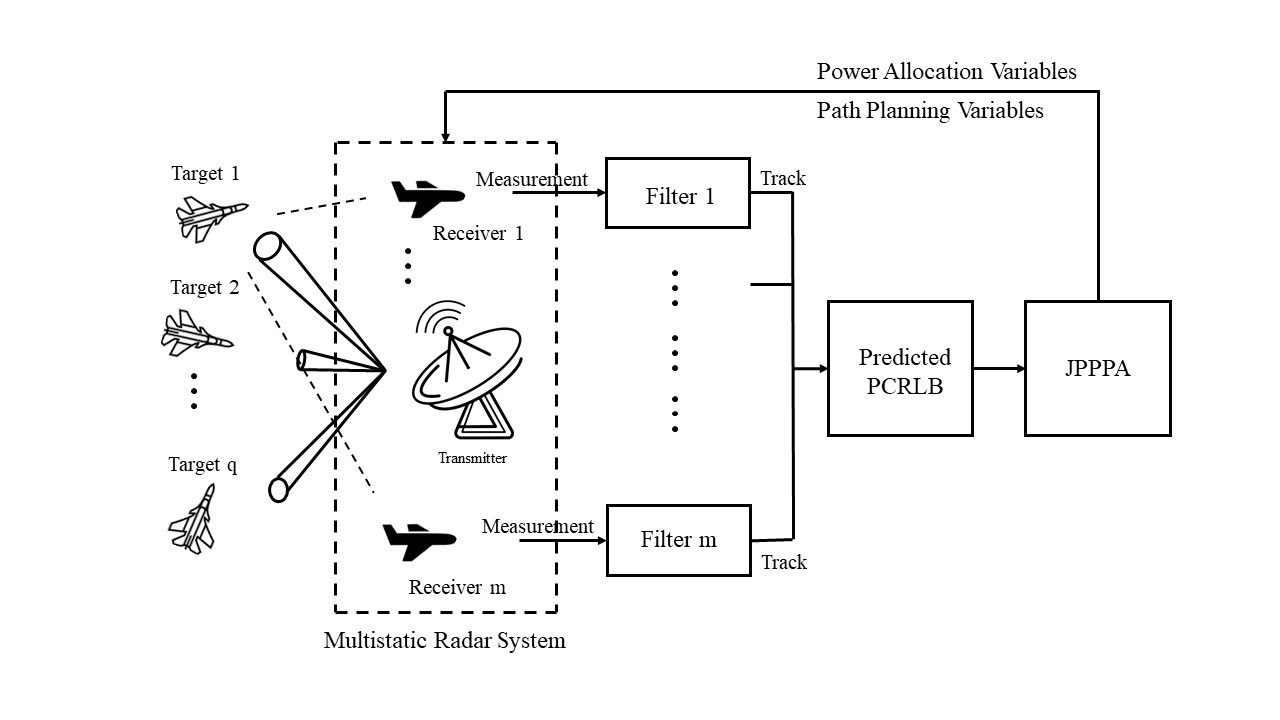
\includegraphics[scale=0.28]{Flow Chart.jpg}
	\caption{JPPPA-based multitarget tracking framework in a multistatic radar system}
	\label{fig:system}
\end{figure}

The remainder of the paper is organized as follows. Section II presents the description of the problem and introduces the system model. The problem is mathematically formulated in Section III. In Section IV, the solution technique of JPPPA optimization problem is presented and a multitarget tracking algorithm based on JPPPA strategy is developed. The simulation results are presented and discussed in Section V and conclusions and  and recommendations are stated in Section VI. 

\section{Problem Description}
Consider a 2-D surveillance area where a multistatic radar system with one transmitter and $N$ receivers is deployed. The position of the transmitter is denoted by $(x_{Tx},y_{Tx})$. The receivers are mounted on UAVs. The $n$th receiver has the initial position $(x_n^1,y_n^1)$, initial velocity $(\dot{x}_n^1,\dot{y}_n^1)$ and initial heading angle $\theta_n^1$. There are $Q$ airborne targets in the surveillance area. The $q$th target is intially located at $(x_q^1,y_q^1)$ with a initial velocity $(\dot{x}_q^1,\dot{y}_q^1)$. At time step $k$, the $q$th target is located at $(x_q^k,y_q^k)$ with velocity $(\dot{x}_q^k,\dot{y}_q^k)$.

For simplicity, it is assumed that the number of targets is fixed and known to the system and all the trackers are already initialized. The multistatic radar should track all the targets in the surveillance area while utilizing limited resources in an efficient manner. The transmitter launches multiple beams that point at different targets simultaneously. The signal to noise ratio (SNR) level %Iyemeh: First mention needs definition. 
of the echoes is proportional to the power radiation that is allocated to generate that beam. Let $P_q^k$ denote the power that is allocated to launch the beam which tracks target $q$ at time step $k$, then we define a power allocation vector $\mathbf{P}_k=[P_1^k, P_2^k,..., P_Q^k]$ %Iyemeh: Shouldn't the k be a superscript to conform with the definitions so far? There are several cases like this in the paper. If it is correct in its current form, ignore the comment.
that denotes the power scheme at time step $k$. 

Meanwhile, the trajectories of UAVs that carry the recievers need to be optimized so that the system may obtain better tracking performance. The maneuver of receiver $n$ at time step $k$ is described by two variables: speed $V_n^k$ and heading angle $\theta_n^k$


\subsection{Signal Model}
The transmitter launches all beams to track different targets simultaneously. The transit beam for target $q$ at time step $k$ is given by the following equation.

\begin{equation}
    s_{n,q}^k(t)=\sqrt{P_{q}^k}E_{n,q}^k(t)exp(-j2\pi f_{c}t)
\end{equation}

where $f_{c}$ is the carrier frequency, and $P_{n,q}^k$ is the transmit power.

The term $E_{n,q}^k(t)$ is the normalized complex envelope of the transmit signal, which has an effective bandwidth of $\beta_{n}$

\begin{equation}
    \beta_{n}^2=\frac{\int f^2|E_{n,q}^k(f)|^2df}{\int |E_{n,q}^k(f)|^2df}
    \label{bandwidth}
\end{equation}

and an effective time duration $T_{q,k}$

\begin{equation}
    T_{n}^2=\frac{\int t^2|E_{n,q}^k(f)|^2dt}{\int |E_{n,q}^k(f)|^2dt}
    \label{time duration}
\end{equation}

The signal received by the $n$th receiver is an attenuated version of the transmit signal, which is delayed by

\begin{equation}
\begin{aligned}
    r_{n,q}^k(t)=&h_{n,q}^k\sqrt{\alpha_{n,q}^{k}P_{q}^k}E_{n,q}^k(t-\tau_{n,q}^k)exp(-j2\pi f_{n,q}^kt)\\
    &+\omega_{n,q}^{k}(t)
\end{aligned}
\end{equation}

The term $\alpha_{n,q}^k \propto{1/(R_{n,q}^k)^4}$ denotes the variation in the signal strength due to loss effects along the signal transmission path (transmitter-target-receiver), %Iyemeh: I have added brackets around transmitter-target-receiver as it does not read right in the current state. It could aslo be "signal transmission path between transmitter-target-receiver". Identify which is appropriate and apply. 
 where $R_{n,q}^k$ is the bistatic, i.e. the sum of the distance from the transmitter to the target and the distance from the target to the receiver. $h_{n,q}^k$ denotes target RCS, also referred to as reflectivity, which is a random variable. $\omega_{q,k}^n$ is a zero-mean complex Gaussian noise.

The time delay is proportional to the bistatic range, given by

\begin{equation}
\begin{aligned}
    \tau_{n,q}^k&=\frac{1}{c}R_{n,q}^k\\
    &=\frac{1}{c}(\left \|(x_{Tx},y_{Tx})-(x_q^k,y_q^k)\right \|+\left \|(x_q^k,y_q^k)-(x_n^k,y_n^k)\right \|)
\end{aligned}
\label{bistatic range}
\end{equation}

where $\left \|\cdot\right\|$ denotes the Euclidean norm. $c$ is the speed of light.

The Doppler shift $f_{n,q}^k$ is proportional to the derivative of the bistatic range, which is given by

\begin{equation} 
	\begin{aligned}
	f_{n,q}^k = - \frac{f_c}{c}& \bigg\{\frac{\dot{x}_q^k\left(x_q^k - x_{Tx} \right) +\dot{y}_q^k \left(y_q^k - y_{Tx} \right)}{\left \|(x_{Tx},y_{Tx})-(x_q^k,y_q^k)\right \|}\\
	&+\frac{\dot{x}_q^k\left(x_q^k - x_n^k \right) +\dot{y}_q^k \left(y_q^k - y_n^k \right)}{\left \|(x_n^k,y_n^k)-(x_q^k,y_q^k)\right \|}\bigg\}
	\end{aligned}
	\label{doppler shift}
\end{equation}


\subsection{Target Dynamics}
Let $\mathbf{x}_q^k={[x_q^k, y_q^k, \dot{x}_q^k, \dot{y}_q^k]^T}$ denote the state vector of the $q$th target, where $\left[ x_q^k, y_q^k \right]$ and $\left[ \dot{x}_q^k, \dot{y}_q^k \right]$ denote the position and velocity of the target, respectively.

The target's motions is assumed to follow a constant-velocity (CV) model in which the state of the target evolves as:
\begin{equation}\ \mathbf{x}_q^{k+1}=\mathbf{F}_k\mathbf{x}_q^k+\mathbf{w}_q^k\end{equation}

$\mathbf{F}_k$ is the transition matrix

\begin{equation}
    {\bf F}_k={\bf I}_{2}\otimes\left[\begin{matrix}1 & T \\ 0 & 1\end{matrix}\right]
\end{equation}

where $\otimes$ is the Kronecker operator, and $\mathbf{I}_2$ denotes the $2\times 2$ identity matrix. $\mathbf{w}^k$ is the process noise that describes the inaccuracy of the motion model. It is assumed to be zero-mean Gaussian distributed with a known covariance $\mathbf{\Gamma}^k$.

The covariance matrix is denoted by

\begin{equation}
    {\bf \Gamma}_{k}=\kappa {\bf I}_{2}\otimes\left[\begin{matrix} {1\over 3}T^{3}&{1\over 2}T^{2}\\ {1\over 2}T^{2}&T\end{matrix}\right]
\end{equation}
%Iyemeh: this term was Ppreviously defined with a superscript, now with a subscript. Confirm and correct if applicable. 
 
where $\kappa$ is the intensity of process noise.
%The transition model of the $i$th target is a first-order Markov process which is described as:
%\begin{equation}
%    \mathbf{h}_k^i=\mathbf{h}_{k-1}^i+\mathbf{\mu}_{k-1}^i
%\end{equation}

%The noise $\mathbf{\mu}_{k-1}^i$ is white Gaussian with a known covariance $\mathbf{Q}_{h,k-1}^i$. The term $\mathbf{h}_k^i=[\mathbf{h}_{1,i,k}^T,\mathbf{h}_{2,i,k}^T,...\mathbf{h}_{N,i,k}^T]^T$ represents the channel state vector ($\mathbf{h}_{j,i,k}=[h_{j,i,k}^R,h_{j,i,k}^I]^T$). Then, the system state vector is extended by concatenating the target state vector and the channel state vector.

\subsection{UAV Kinematic Model}
UAVs are constrained by their kinematic capacities. In this paper, a 2-D maneuvering model is used. The heading angle and speed of each UAV might change at each observation time point, while within the time interval, the UAVs are assumed to move in a constant velocity with their heading angles and speeds fixed. 

Let $\theta_n^k$ and $V_n^k$ denote the heading angle and the speed of the $n$th receiver at time step $k$, then the position of this receiver $[x_n^k, y_n^k]^T$ evolves as:

\begin{equation}
    [x_n^k, y_n^k]^T=[x_n^{k-1}, y_n^{k-1}]^T+V_n^kT[cos(\theta _n^k), sin(\theta _n^k)]^T
    \label{UAV model}
\end{equation}

where $T$ is the time interval.

At each time step, the maneuver of each UAV must satisfy the kinematic constraints, i.e., the acceleration and the angular acceleration must be within a specified interval, given by:

\begin{equation}
    \left\{
    \begin{array}{lr}
    |\theta_n^k-\theta_n^{k-1}|\leq \theta_{max}
    \\|V_n^k-V_n^{k-1}|\leq a_{max}
    \end{array}
    \right.
    \label{UAV constraints}
\end{equation}

$\theta_{max}$ and $a_{max}$ are the maximum angular and linear accelerations of each UAV, which are assumed to be constants.

\subsection{Measurement Model}
In a general case where there exists measurement origin uncertainty(MOU), measurements originate from one of the targets or from clutter. The measurement is given by:

\begin{equation}
    \mathbf{z}_{n,q}^k=\begin{cases} h_{n}(\mathbf{x}_q^k)+\mathbf{w}_{n,q}^k & \mbox{if originated from target}\ q\\ \upsilon_{n,q}^k & \mbox{if false alarm}
    	\end{cases}
    \label{measurement function}
\end{equation}

where $\mathbf{z}_{n,q}^k$ is the measurement of target $q$ at time step $k$ that is obtained by the $n$th receiver, $h_{n}$ is the nonlinear observation function. The measurements consist of bistatic range $R_{n,q}^k$, bearing from target to sensor $\theta_{n,q}^k$, and Doppler shift $f_{n,q}^k$, i.e.,

\begin{equation}
	h_{n}(\mathbf{x}_q^k)=[R_{n,q}^k, \theta_{n,q}^k, f_{n,q}^k]^T
\end{equation}

The bearing is given by:

\begin{equation}
\theta_{n,q}^k=\arctan {(\frac{{y_{n,q}^k - y_n^k}}{{x_{n,q}^k - x_n^k}})} 
\end{equation}

and the expressions of $R_{n,q}^k$ and  $f_{n,q}^k$ can be found in equations (\ref{bistatic range}) and (\ref{doppler shift}).

$\mathbf{w}_{n,q}^k$ is the measurement noise, which is assumed to be a zero-mean Gaussian random variable with covariance $\mathbf{\Sigma}_{n,q}^k$. 

\begin{equation} 
\boldsymbol {\Sigma}_{n,q}^k = \text{diag}\left({\sigma _{R_{n,q}^k}^2,\sigma _{\theta _{n,q}^k}^2,\sigma _{f_{n,q}^k}^2} \right)
\label{measurement noise covariance}
\end{equation}

where $\sigma _{R_{n,q}^k}^2$, $\sigma _{\theta _{n,q}^k}^2$ and $\sigma _{f_{n,q}^k}^2$ are the CRLBs %Iyemeh: first mention, except if it has the same definition as PCRLB.
on the estimation MSE of the $q$th target's bistatic range, bearing and Doppler shift estimates, which satisfy

\begin{equation}
	\begin{cases}
		\sigma _{R_{n,q}^k}^2 \propto {\left(\mu_{n,q}^k{\beta _n^2} \right)^{ - 1}}\\ 
		\sigma _{\theta _{n,q}^k}^2 \propto {\left(\mu_{n,q}^k/{B_{W}} \right)^{ - 1}} \\
		\sigma _{f_{n,q}^k}^2 \propto {\left(\mu_{n,q}^kT_n^2 \right)^{ - 1}}
	\end{cases}
\label{R}	
\end{equation}

where $B_W$ is the null-to-null width of the receiver antennas, $\beta _n$ and $T_n$ are the effective bandwidth and time duration of the transmit signal previously defined in (\ref{bandwidth}) and (\ref{time duration}). $\mu_{n,q}^k$ is the SNR which satisfies $\mu_{n,q}^k \propto \alpha _{n,q}^k P_{q}^k {\left| {h_{n,q}^k} \right|}^2$, thus we have

\begin{equation}
     \begin{cases}
     	\sigma _{R_{n,q}^k}^2 \propto {\left({\alpha _{n,q}^k P_{q}^k {{\left| {h_{n,q}^k} \right|}^2}{\beta _n^2}} \right)^{ - 1}}\\ 
     	\sigma _{\theta _{n,q}^k}^2 \propto {\left({\alpha _{n,q}^k P_{q}^k {{\left| {h_{n,q}^k} \right|}^2}}/{B_{W}} \right)^{ - 1}} \\
     	\sigma _{f_{n,q}^k}^2 \propto {\left({\alpha _{n,q}^k P_{q}^k {{\left| {h_{n,q}^k} \right|}^2}T_n^2} \right)^{ - 1}}
     \end{cases}
\end{equation}

Note that the elements in (\ref{R}) are inversely proportional to the allocated power $P_{q}^k$, which yields an intuitive conclusion that for a single target, the covariance of the measurement noise is inversely proportional to the power that is assigned to track it, i.e., the more power assigned to track a target, the more accurate the measurements of that target will be.

The term $\upsilon_{n,q}^k$ in(\ref{measurement function}) represents the measurement generated by clutters, which is a zero-mean Gaussian random variable uniformly distributed in the measurement space (within the observation volume $V$). The number of false alarms at each frame satisfies Poisson distribution, given by 

\begin{equation}
	p(n_{fa})=\frac{e^{-\lambda V}(\lambda V)^{n_{fa}}}{n_{fa}!}
\end{equation} 

where $n_{fa}$ is the number of false alarms, $\lambda$ is the spatial density, i.e., the average number of false alarms at each frame.

\subsection{FIM and PCRLB}
The Posterior Cramér-Rao lower bound (PCRLB), which is defined to be the inverse of Fischer information matrix (FIM), gives a lower bound of the error covariance matrix of a unbiased estimate. It gives a measure of the achievable optimum performance and can be calculated
predictively. Furthermore, the PCRLB is independent of the filtering algorithm, thus is often used as an effective criterion in optimal sensor resource management problems. For simplicity, the receiver index $n$ is omitted in this subsection. Let $\hat{\mathbf{x}_k}$ be an unbiased estimate of $\mathbf{x}_k$ based on the measurement $\mathbf{z}_k$, $\mathbf{C}_k$ be the error covariance matrix, and $\mathbf{J}(\mathbf{x}_k)$ be the FIM, we have 
\begin{equation}
    \mathbf{C}_k=\mathbb{E}[(\hat{\mathbf{x}}_k-\mathbf{x}_k)(\hat{\mathbf{x}}_k-\mathbf{x}_k)^{T}]\geq \mathbf{J}_(\mathbf{x}_k)^{-1}
\end{equation}

where $\mathbb{E}$ denotes expectation operator.

A decent recursive formula for the calculation of PCRLB is developed in\cite{tichavsky1998posterior}

\begin{equation}
	\mathbf{J}_k=\mathbf{J}_X(\mathbf{x}_k)+\mathbf{J}_Z(\mathbf{x}_k)
	\label{J}
\end{equation}

where $\mathbf{J}_X(\mathbf{x}_k)$ and $\mathbf{J}_Z(\mathbf{x}_k)$ are the prior knowledge and the information obtained from measurements at time step $k$ respectively.

\begin{equation}
	\begin{cases}
		\mathbf{J}_{X}(k)=\mathbf{D}_{k-1}^{33}-\mathbf{D}_{k-1}^{21}(\mathbf{J}_k+\mathbf{D}_{k-1}^{11})^{-1}\mathbf{D}_{k-1}^{12}\\
		\mathbf{J}_Z(k) =\mathbb{E}\{-\Delta _{\mathbf{x}_{k}}^{\mathbf{x}_{k}}\ln p(\mathbf{z}_k|\mathbf{x}_{k})\}
	\end{cases}    
\end{equation}

where
\begin{equation}
	\begin{cases}
		\mathbf{D}_{k-1}^{11}=\mathbb{E}\{-\Delta _{\mathbf{x}_{k-1}}^{\mathbf{x}_{k-1}}\ln p(\mathbf{x}_k|\mathbf{x}_{k-1}\}\\
		\mathbf{D}_{k-1}^{12}=\mathbb{E}\{-\Delta _{\mathbf{x}_{k}}^{\mathbf{x}_{k-1}}\ln p(\mathbf{x}_k|\mathbf{x}_{k-1}\}=(\mathbf{D}_{k-1}^{21})^T\\
		\mathbf{D}_{k-1}^{22}=\mathbb{E}\{-\Delta _{\mathbf{x}_{k}}^{\mathbf{x}_{k}}\ln p(\mathbf{x}_k|\mathbf{x}_{k-1}\}
	\end{cases}   
\end{equation}   

The prior information is given by
\begin{equation}
    \mathbf{J}_X(\mathbf{x}_k)=[\mathbf{\Gamma}_{k-1}+\mathbf{F}_k\mathbf{J}(\mathbf{x}_{k-1})^{-1}\mathbf{F}_{k-1}^T]^{-1}
\end{equation}

It is assumed that the measurements collected from different bistatic pairs are independent, hence, the total measurement contribution is equal to the summation of measurement contributions obtained by all bistatic pairs.

\begin{equation}
    \mathbf{J}_Z(\mathbf{x}_k)=\sum_{n=1}^N\mathbf{J}_{Z_{n}}(\mathbf{x}_k)
\end{equation}

The measurement contribution obtained by a single bistatic pair is given by
\begin{equation}
    \mathbf{J}_{Z_{n}}(\mathbf{x}_k)=\mathbb{E}\{q(\mathcal{P}_{n,q}^k,\Sigma_{q,k})\mathbf{H}_{q,k}^T\Sigma_{q,k}^{-1}\mathbf{H}_{q,k}\}
    \label{Jz}
\end{equation}

where $\mathbf{H}_{q,k}=[\Delta_{\mathbf{x}_q^k}h_n^T(\mathbf{x}_q^k)]^T$ is the Jacobian matrix of the measurement function $h_n(\mathbf{x}_q^k)$ with respect to the target state $\mathbf{x}_q^k$. and $\mathbb{E}$ denotes expectation with respect to the target state. The term $q(\mathcal{P}_{n,q}^k,\Sigma_{q,k})$ is the information reduction factor (IRF)\cite{niu2001matrix} which modifies the information obtained from measurements due to MOU. The reader is referred to \cite{tharmarasa2007pcrlb,hernandez2004multisensor} for details about IRF.

This expected value in (\ref{Jz}) can be calculated through Monte Carlo techniques, but it will cause extra computational cost. To maintain efficiency in real time applications, the measurement contribution can be approximcated using the Jacobian and measurement noise covariance evaluated at the prediction phase.

\begin{equation}
	\mathbf{J}_{Z_{n}}(\mathbf{x}_k)=q(\mathcal{P}_{n,q}^k,\Sigma_{q,k})\mathbf{H}_{q,k}^T\Sigma_{q,k}^{-1}\mathbf{H}_{q,k}\bigg|_{\mathbf{x}_{k|k-1}^q}	
\end{equation}

where $\mathbf{x}_{k|k-1}^q$ denotes the predicted state of the $q$th target at time step $k$. 

Substituting the prior information and measurement contributions into (\ref{J}), we can get the predicted FIM as

\begin{equation}
	\begin{aligned}
	\mathbf{J}|_{\mathbf{x}_k}=&[\mathbf{\Gamma}_{k-1}+\mathbf{F}_k\mathbf{J}(\mathbf{x}_{k-1})^{-1}\mathbf{F}_{k-1}^T]^{-1}\\
	&+\sum_{n=1}^{N}[q(\mathcal{P}_{n,q}^k,\Sigma_{q,k})\mathbf{H}_{q,k}^T\Sigma_{q,k}^{-1}\mathbf{H}_{q,k}]\bigg|_{\mathbf{x}_{k|k-1}^q}
	\end{aligned}
    \label{eqn:predicted FIM}
\end{equation}

Note the power allocation scheme changes the FIM through $\Sigma_{q,k}$ and the path planning variables change the FIM through $\mathbf{H}_{q,k}$.

Then, the predictive PCRLB is defined to tthe inverse of FIM:

\begin{equation}
	\mathbf{C}_{PCRLB} = (\mathbf{J}|_{\mathbf{x}_k})^{-1}
\end{equation} 

\section{Optimization Formulation}
At every time step $k$, decisions need to be made on the power allocation scheme of the transmitter and the maneuver of each receiver, which is controlled by its heading angle and speed. The decision variables are displayed as follows:

\begin{equation}
    \left\{
    \begin{array}{lr}
    \mathbf{P}_k=[P_1^k, P_2^k,..., P_Q^k]^T
    \\\mathbf{V}_k=[V_1^k, V_2^k,..., V_N^k]^T
    \\\mathbf{\Theta}_k=[\theta_1^k, \theta_2^k,..., \theta_N^k]^T
    \end{array}
    \right.
\end{equation}

The PCRLB is used as a criterion to be minimized, hence the trace of PCRLB is taken as a scalar metric.

\subsection{Objective}
The diagonal elements of the PCRLB matrix are the lower bounds on the estimation MSE of the target position and velocity. To minimize such lower bounds, the trace of the PCRLB matrix is selected as the objective to minimize. The PCRLB is obtained by taking the inverse of FIM. 

\begin{equation}
    \min\ (\mathbf{J}|_{\mathbf{x}_q^k})^{-1}
\end{equation}

Since the information of all targets obtained from all bistatic pairs are independent, the goal of the JPPPA optimization is to minimize the summation of the traces of all PCRLB matrices, i.e., the summation of lower bounds on the estiamtion MSE of all targets, which is given by

\begin{equation}
    U_k(\mathbf{P_k},\mathbf{V_k},\mathbf{\Theta_k})=\sum_{q=1}^Q(\mathbf{J}|_{\mathbf{x}_q^k})^{-1}
\end{equation}

In some works\cite{xie2017joint}, only the position RMSE %Iyemeh: First use, needs definition
 is considered, which is an alternative objective since the position RMSE is generally much larger than the velocity RMSE. In that case, the objective function is defined as the summation of first and the third elements on the diagonal of the PCRLB matrix, which represent the lower bounds on the estimation errors of position in $x$ and $y$ coordinates, respectively.

\subsection{Constraints}
1) \emph{Constraints on UAVs' maneuverability:} The UAVs are constrained by their kinematic capabilities. The path planning variables, which are heading angles and speeds, have upper and lower limits, given by 

\begin{equation}
	\left\{
	\begin{array}{lr}
		|V_n^k-V_n^{k-1}|\leq a_{max}
		\\|\theta_n^k-\theta_n^{k-1}|\leq \theta_{max}
	\end{array}
	\right.
	\label{UAV maneuverability}
\end{equation}

$\theta_{max}$ and $a_{max}$ are the maximum angular and linear accelerations.

A minimum and a maximum speed of UAVs are also defined to maintain the UAVs' speeds in a reasonable range if a UAV receives consecutive acceleration/deceleration commands.

\begin{equation}
	V_{min}<V_n^k<V_{max}
	\label{UAV speed}
\end{equation}

where $V_{min}$ and $V_{max}$ are the minimum and maximum speeds.

2) \emph{Constraints on power budget:} The summation of power allocated to all beams must not exceed the total power budget, denoted as:

\begin{equation}
	{{\mathbf 1}^T}{{\mathbf P}_k}={P_{\text{total}}}
	\label{total power budget}
\end{equation}

Each power radiation is constrained by a minimum value $P_{min}$ to ensure sufficient signal intensity for a detection, and a maximum value $P_{max}$ to ensure reasonable allocation to other beams.

\begin{equation}
	P_{min}\leq P_{k,m}^q\leq P_{max}
	\label{power range}
\end{equation}

Mathematically, a beam with very weak power radiation will make corresponding covariance of measurement noise (\ref{measurement noise covariance}) close to singular, which will be avoided by the power constraint.

Since the power radiations and speeds of UAVs are not direct decision variables, constraints (\ref{UAV speed}) and (\ref{power range}) may be violated during the optimization process. Penalty functions are defined to restrain these variables within their constrained ranges.

The penalty function for constraint (\ref{UAV speed}) is expressed as

\begin{equation}
	\begin{aligned}
		\mathcal{F}_1(k) = \mathcal{U}&\sum_{n=1}^{N}[\max\ (|V_{max}-V_n^k|,0)+\\
		&\max\ (|V_{min}-V_n^k|,0)]
	\end{aligned}	
\end{equation}

where $\mathcal{U}$ is a large positive constant.

Similarly, the penalty function for constraint (\ref{power range}) is expressed as

\begin{equation}
	\begin{aligned}
		\mathcal{F}_2(k) = \mathcal{U}&\sum_{q=1}^{Q}[\max\ (|P_{max}-P_q^k|,0)+\\
		&\max\ (|P_{min}-P_q^k|,0)]
	\end{aligned}	
\end{equation}


%A minimum distance between a UAV and the target is defined for safety purposes.
%\begin{equation}
%    \|[x_k^i, y_k^i]-[x_k, y_k]\|\geq d_{R-T}
%\end{equation}

%Similarly, a minimum distance between two different UAVs is defined to avoid collision.
%\begin{equation}
%    \|[x_k^i, y_k^i]-[x_k^j, y_k^j]\|\geq d_{R-R},\ i\neq j
%\end{equation}

%A maximum distance between two different UAVs is also defined to ensure that the receivers stay in communication. Usually this is a soft constraint that cannot be easily violated.

\subsection{Receding Horizon Control}
Receding horizon control (RHC) framworks have been popular for the control of UAVs. By extending a one-step optimization to a control sequence, these approaches offer the potential of responding to a dynamic environment\cite{frew2005receding} with increase in computational cost.
Since the UAVs are constrained by their kinematic capabilities, the controlling decision made on UAVs at time step $k$ $(\mathbf{V}_k,\mathbf{\Theta}_k)$ will affect the future moves. Therefore, it is practical and technically useful to consider future steps instead of performing only a greedy one-step optimization.
The weighted sum of predicted worst-case PCRLB in the next $H$ steps is given below.

\begin{equation}
	\sum_{h=1}^{H}w_{k+h}U_{k+h}=\mathbf{W}_k^T\mathbf{U}_k
\end{equation}

where $\mathbf{W}_k=[w_{k+1}, w_{k+2},...,w_{k+H}]^T$ is the vector of weights on predicted worst-case PCRLBs, also referred to as receding horizon decay factors.

\emph{Remark 1:} Since the hard constraints (\ref{UAV speed}) and (\ref{power range}) are tranformed into penalty functions and added to the objective function, it is possible that these constraints might be violated due to the long-term multi-step planning of RHC. This can be avoided by increasing the penalty factor $\mathcal{F}$.

When the fitness value is being evaluated, the updated tracks from previous time step are required to predict the current states of targets which are needed in the predictive PCRLB. When we plan for future steps in the receding horizon control sequence, such updated tracks will not be available. To handle this, we use predicted tracks from previous time step to do the prediction as if no valid measurements were obtained.

\emph{Remark 2:} RHC is most suitable in obstable avoidance\cite{frew2005receding} where the environment is dynamic. While it introduces extra computational load without being able to significantly improve the optimization result, it is still meaningful to apply RHC in our case. Sending sequenced commands to UAVs is advantageous over continuously sending one-step commands due to possible communication failure or other unexpected situations.

\subsection{Problem Formulation}
By adding the weighted sum of PCRLB at all time steps in the RHC sequence with the penalty functions, the objective function of the JPPPA optimization is obtained.

\begin{equation}
	\mathbb{F}(\mathbf{P_k},\mathbf{V_k},\mathbf{\Theta_k})=\mathbf{W}_k^T\mathbf{U}_k + \mathcal{F}_1 + \mathcal{F}_2
\end{equation}

The optimization problem is summarized as

\begin{align} 
\min \quad & \mathbb{F}(\mathbf{P_k},\mathbf{V_k},\mathbf{\Theta_k})\nonumber\\ s.t.\quad & {{{\mathbf 1}^T}{{\mathbf P}_k}={P_{\text{total}}}} \nonumber\\ & P_{min}\leq P_{k,m}^q\leq P_{max}\nonumber\\ &|V_n^k-V_n^{k-1}|\leq a_{max} \nonumber\\ &|\theta_n^k-\theta_n^{k-1}|\leq \theta_{max}\\ &V_{min}<V_n^k<V_{max} . 
\label{problem}
\end{align}

\section{Joint Path Planning and Power Allocation Strategy}


\subsection{Solution Technique Based on Genetic Algorithm}
From previous sections, it can be seen that the optimization problem (\ref{problem}) is nonconvex due to the complexity of the objective function and operations that change convexity such as the trigonometric functions in (\ref{UAV model}). It is hard to solve this problem, which is NP-hard, through convex optimization techniques. Hence, a genetic algorithm (GA) with custom operator was developed.  

Genetic algorithm is an evolutionary searching technique inspired by natrual selection.%Iyemeh: include a reference
 The decision variables in the solution space are represented as individuals (also referred to as chromosomes). By eliminating individuals with low fitness values, genetic algorithm has a strong capability of global search, however it does not offer a good local search performance. In the scenario where the receivers await their moving commands at each time step, the decision variables must be determined online in limited time. Therefore, it's desirable to obtian a sub-optimal solution as fast as possible rather than to spend extra time searching for the global optimal solution wherein the improvement may not be signifinicant.

The individuals are structured as follows: for each time step, the first $Q$ genes represent the power radiations that are allocated to $Q$ targets and the rest genes represent the path planning variables (speeds and heading angles). The same structure repeats for every time step that is in the receding horizon control sequence. The total length of a single individual is $H(Q+2N)$. The power radiations are random numbers from 0 to 1 that satisfy constraint (\ref{total power budget}) when generated. For simplicity, the speeds and heading angles are mapped to continous values from 0 to 1. The mapping functions are given by 

\begin{equation}
	\bar{V}_n^k=\frac{V_n^k+a_{max}}{2a_{max}}, \  \bar{\theta}_n^k=\frac{\theta_n^k+\theta_{max}}{2\theta_{max}} 
\end{equation}

When evaluating the fitness value of an individual, these intermediate values are converted back to real ones.

\emph{Remark 3:} A proper encoding method is vital to the performance of GA. In this work, real number encoding where each decision variable is represented by one gene is adopted. Gray encoding is more suitable for local search because the randomness introduced in crossover and mutation operations is smaller. However, its encoding efficiency is low since a decision variable is represented by multiple binary genes. Therefore, the computational cost is increased due to the large chromosome length. Numerical experiments in this case showed that gray encoding offered worse integral performance. 

Individuals are evaluated and updated through the selection operation, where the traits of two parent chromosomes are exchanged to breed new offsprings. Those with high fitness values are more likely to be selected and copied to the next generation, while those with low fitness values will be eliminated. Roulette wheel and tournament schemes are the most used strategies for selection.%Iyemeh: reference needed to support this point
 To protect the elite individuals, a binary tournament selection is adopted in this paper. 

The information of the population is shared and exchanged in the crossover operation. When crossover is performed, a random locus is selected, then the genes before and after that locus are exchanged between two chromosomes. 

To maintain the diversity of the population, mutation operation is performed. Each gene has a small probability $P_m$ to mutate. Binary variables are flipped and continous variable are replaced by a random value. In our case where all the genes are continous variables, they will mutate to a random value between 0 and 1.

In the crossover and mutation operations, the power constraint (\ref{total power budget}) may be violated, hence, a repair operation is provided to rectify infeasible individuals. If the summation of power radiations are not equal to 1, the whole power scheme will be scaled so that the power constraint is met.

Elitism is adopted to protect highly fitted individuals. A few individuals with high fitness value are preserved after the selection operation and are directly copied to the next generation without participating in the crossover and mutation operations. Elitism prevents the losing of top-ranked individuals and preserves fitted genes which might improve the performance of the algorithm. %Iyemeh: Reference required if paraphrased from literature. 

The population keeps evolving until some termination conditions are met, e.g., the maximum number of iteration is reached or there is no improvement found in the population for a certain number of generations.

%Iyemeh: I have rephrased this sentence as it is a bit confusing. "Starting from the second step, the JPPPA decision on this step that was obtained in the previous receding horizon control sequence will become available under the RHC framework."
From the second step, the JPPPA decision is based on the previous receding horizon control sequence and it will become available under the RHC framework. The previously obtained decision will be referred to as a \emph{prior}. Since the prior was already a near-optimal solution, taking advantage of it will significantly improve the structure of the population and reduce the computational cost.
Based on the prior information, we develop a pre-selection operator that will replace the normal population generation.

The pre-selection operation includes the following steps:

1) \emph{Generate the elite individual:} Generate random sets of genes that represent the decision variables at the last time step in the current RHC sequence (where there is no prior available). Combine the random genes with the prior to generate new individuals. Find the fittest one among those individuals and preserve it as an elite.

2) \emph{Generate population:} Randomly generate individuals and put them together with the elite to establish a population.

3) \emph{Small-scale crossover:} Choose the elite individual as a parent and crossover with other individuals.

4) \emph{Small-scale mutation:} Mutate the elite individual. In this phase, genes to be mutated are not replaced by a random value, but an increment that satisfies a zero-mean Gaussian distribution will be added. i.e., the mutated individuals are more likely to be around the elite in the solution space.

5) \emph{Repair and replace:} Repair the individuals generated from previous crossover and mutation. Use them to replace random individuals.

By essentially changing the structure of the population, the pre-selection operator achieves the aim of \emph{providing guidance to the randomly generated population} and \emph{searching the space around the prior information}. This operation is equivalent to giving more weight to the prior information and can be seen as an extra generation of the evolution. Note the pre-selection is performed only once at each time step. Limited time is spent to crossover and mutate the elite individual that could breed better offsprings. To preserve the population's diversity that may be reduced by the pre-selection operation, only a limited portion of individuals will be replaced. 

\begin{figure}
	\centering
	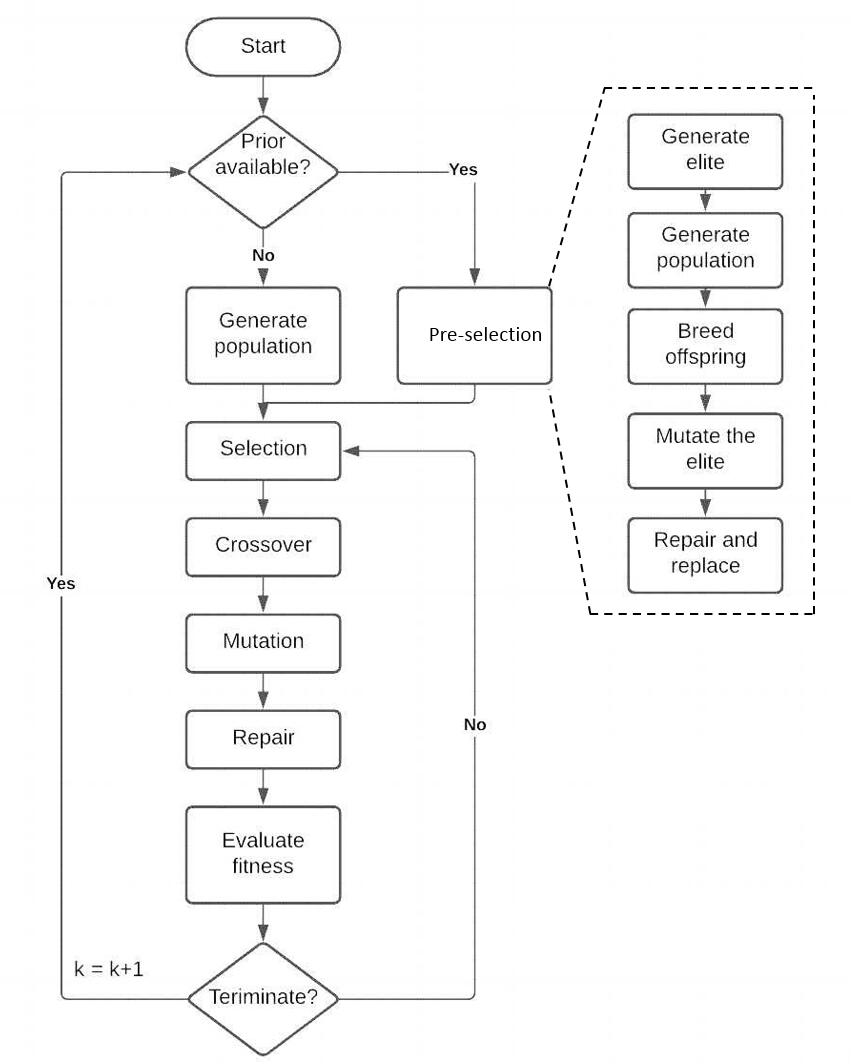
\includegraphics[scale=0.36]{GA.jpg}
	\caption{Flow chart of the modified genetic algorithm with custom pre-selection operator}
	\label{fig:GA}
\end{figure}
\subsection{Multiple Target Tracking}

 It is assumed that the targets are widely separated in the surveillance area. Therefore, after the decisions are made by the JPPPA strategy, the multitarget tracking problem becomes several single target tracking problems that can be handled independently.
%Iyemeh: There should be a sentence to link next paragraph with the previous paragraph. Maybe something like:
To handle independent tracking for serveral targets, Particle filter (PF) is used. 

Particle filter (PF) has a strong potential when dealing with nonlinear measurements \cite{arulampalam2002tutorial}. In this paper, the measurement equations are highly nonlinear, hence a particle filter is an ideal choice.

The particle filter is a Monte Carlo technique that represents the density $p(\mathbf{x_k|z_k})$ as a random set of samples (particles) $\lbrace \mathbf{x}_k^p:p=1,...,P \rbrace$ with corresponding weights  $\lbrace w_k^p:p=1,...,P\rbrace$. At each time step, particles are generated by sampling from the prior. Then, they are predicted and updated under the Bayesian filtering framework. The weight of each particle is updated correspondingly after measurements are collected. Finally, resampling is performed to eliminate particles with low weights. In this paper, a Sampling Importance Resampling (SIR) is used as the resampling strategy. A breif summary of SIR-PF is given in Algorithm 1. Note that, other nonlinear filters can also be used, for example, the extended Kalman filter (EKF)\cite{bar2004estimation}. 



\begin{algorithm}
\caption{Multi-target Tracking with JPPPA} 
\label{alg:Framwork} 
\begin{algorithmic}[1]
\STATE Let $k=1$; assume initial JPPPA decisions; assume initial density $p(\mathbf{x}_{k-1})$
\STATE Sample $N_p$ particles from the prior $p(\mathbf{x}_{k|k-1})$ and define corresponding weights.
\FOR{each $q \in [1,Q]$}
\STATE Obtain measurements in the environment that is determined by the JPPPA decisions.
\STATE Update particles' weight based on the posterior $p(\mathbf{x}_k|\mathbf{z}_k)$.
\STATE Resample with SIR strategy and perform weight normalization.
\STATE Calculate the estimation based on particles and weights.
\ENDFOR
\STATE Formulate the JPPPA optimization problem (\ref{problem}) and solve it with the proposed GA.
\STATE Let $k=k+1$, and go to step 3.
\end{algorithmic}
\end{algorithm}

The entire signal processing framework that incorporates a JPPPA optimization module and a particle filter is structured as follows. First, the estimated state of each target is obtained by PF. Then, based on the estimated tracks, the predictive PCRLB is evaluated by JPPPA and optimal resource management deployment is obtained. Finally, the resource management decisions are sent back to the transmitter and recievers to guide their behaviors in the next few steps.

\subsection{Analysis of Computational Complexity}
The computational complexity of GA depends on the size of individuals, the population size and the number of generations, while the size of individuals is determined by the size of the problem, i.e., the number of transmitters, receivers and targets and the length of the RHC sequence. The complexity is on the order of $\mathcal{O}(gpL(MQ+2N))$, where $g$ is the number of generations, $p$ is the population size and $L$ is the length of the RHC sequence. The size of the problem increases the complexicity by the order of 3 at most. The complexity arises from the enlarged size of individuals. Note that in this paper, the number of transmitters $M=1$. 

%Although the computational complexity of GA is decent, it is noteworthy that the performance of GA will degrade as the structure of chromosomes become longer and more complex. When the scale of the problem is large, GA may   

However, the complexity given above is the maximum one where the generation of the population reaches its maximum limit. Generally, the population will quit evolving if no improvement is found for a certain value of generations. Therefore, the performance of GA cannot be evaluated simply by its complexity. The custom pre-selection operator which improves the distribution of individuals can make the population converge faster, although it does not change the maximum complexity. The evaluation of the pre-selection operator is presented in the next section.

\section{Simulation Results and Discussion} %Iyemeh: This should updated to Result and Discussion
 A multistatic radar with one transmitter and $N=5$ movable receivers is considered. The area is surveilled for 30 frames with the time interval $\Delta T = 1$s. The signal effective bandwidth and effective time duration are set to $\beta_n=1$ MHz and $T_n=1$ ms, respectively. The carrier wavelength $\lambda=0.2$ m. The detection probability $\mathcal{P}_{n,q}^k$ is modeled as a function of bistatic range\cite{sinha2005autonomous}. The lower and upper bounds for power constraints are $P_{min}=0.1P_{total}$ and $P_{max}=0.8P_{total}$, respectively. The maximum linear and angular accelerations per frame are set to $a_{max}=300$ m$/$s$\cdot\Delta T$ and $\theta_{max}=15^\circ / \Delta T$, respectively. The lower and upper bounds for UAVs' speed are $V_{min}=200$ m$/$s and $V_{max}=400$ m$/$s. $Q=5$ targets are widely seperated in the surveillance region with $\kappa=50$m$^2/$s$^3$ for all targets. The initial states of targets  and receivers are given respectively in Table \ref{tab:Target State} and Table \ref{tab:Receiver State}%Iyemeh: Table I and II should come before Fig. 4 in the paper as they are discussed before the figure. Try holding the positions of the tables on LaTex.
. The transmitter is located at the origin. Fig. %Iyemeh: Figure reference missing
illustrates the trajectories of targets and the initial radar deployment.

\begin{figure}
	\centering
	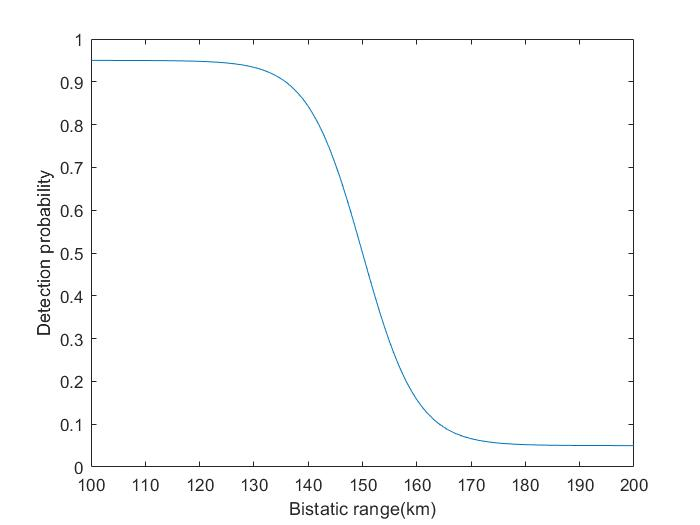
\includegraphics[scale=0.36]{Pd.jpg}
	\caption{Detection probability with respect to bistatic range}
	\label{fig:pd}
\end{figure}
%Iyemeh: This figure was not discussed in the paper. 

The population of GA is 101. The probabilities of crossover and mutation are set to $P_c=0.6$ and $P_m=0.1$, respectively. The maximum generation is 30. The GA terminates when the maximum generation is reached or when there is no improvement in the population for 5 generations. All the results are averaged over 100 Monte Carlo runs.

\begin{figure}
	\centering
	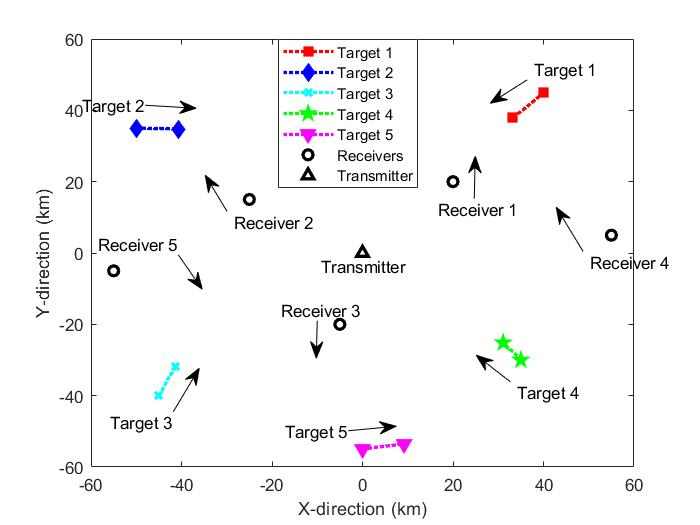
\includegraphics[scale=0.36]{Initial State.jpg}
	\caption{Target trajectories and initial radar deployment}
	\label{fig:pd}
\end{figure}

 \begin{table}
	\centering
	\caption{Initial Target States}
	\begin{tabular}{ccc}
		\toprule
		Target Index & Position (km) & Velocity (m/s)\\ \midrule
		1 & (40,45) & (-200,-250)\\ 
		2 & (-50,35) & (300,0)\\ 
		3 & (-45,-40) & (100,250)\\ 
		4 & (35,-30) & (-150,200)\\ 
		5 & (0,-55) & (250,50)\\ 
		\bottomrule
	\end{tabular}
\label{tab:Target State}
\end{table} 

 \begin{table}[H]
	\centering
	\caption{Initial Receiver States}
	\begin{tabular}{cccc}
		\toprule
		Receiver Index & Position (km) & Speed (m/s) & Heading Angle ($^\circ$)\\ \midrule
		1 & (20,20) & 300 & 90\\ 
		2 & (-25,15) & 300 & 120\\ 
		3 & (-5,-20) & 300 & 270\\ 
		4 & (55,5) & 300 & 120\\ 
		5 & (-55,-5) & 300 & 240\\ 
		\bottomrule
	\end{tabular}
\label{tab:Receiver State}
\end{table}

\subsection{Demonstration of the JPPPA Strategy}
The JPPPA strategy is compared to a two-step algorithm that incorporates typical algorithms in path planning\cite{hernandez2004optimal} and power allocation\cite{yan2016joint} respectively.

In step one, we assume the power scheme remains the same as the last time step. Then, the solution space is discretized and a dynamic programming (DP) is used to find the optimal path planning decisions. Due to the high complexity of DP, the searching technique proposed in \cite{hernandez2004optimal} is used. Note that DP is applied in dynamic environments under the RHC framework, it reduces to greedy search if the problem is a one-step planning.

After the optimal sensor deployment is obtained, the succeeding power allocation problem is convex\cite{boyd2004convex} and thus can be solved with basic optimization techniques. In this simulation, a pattern search technique\cite{koohifar2016receding} is used to find the optimal solution. Pattern search searches the solution space in pre-defined directions. Since it is not required to determine the gradient or the step length, pattern search is suitable in this scenario.

This two-step algorithm is referred to as DP-LS. %Iyemeh: First mention, define acronym.

\emph{Remark 4:} Since the power allocation problem with a fixed receiver deployment is convex, it can be solved easily, e.g., with the CVX toolbox and no advanced algorithm is required. In fact the gradient projection (GP) used in (\ref{total power budget}) is a favorable solution due to the existence of equality constraints. However, in the proposed scenario, the gradient is hard to determine due to the large scale of the problem. Several similar works have made contributions on transforming or relaxing their original problems into the convex one that is easy to solve%Iyemeh: Add reference
. This approach, however, is infeasible in the proposed case due to the complexity of objective function introduced by sensor mobility.

The proposed JPPPA strategy are also compared with the following strategies:

1) \emph{One-step JPPPA} (1-JPPPA): The same alogorithm is adopted except that RHC is not considered. At each time step, the solver only seeks the decision variables for the next frame without considering the future.

2) \emph{Uniform Power Allocation} (UPA): By assuming the power is uniformly allocated to all targets, the joint optimization degrades into a pure path planning, which is also nonconvex.

Fig. \ref{fig:PCRLB} displays the real PCRLB values after the optimization result is obtained.

\begin{figure}
	\centering
	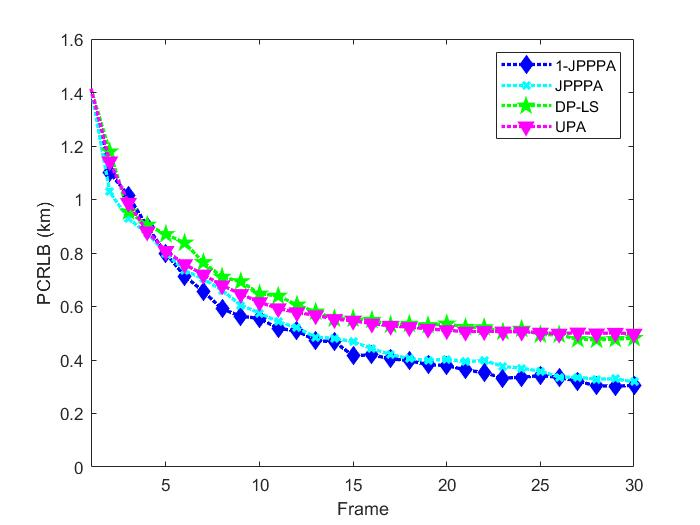
\includegraphics[scale=0.36]{PCRLB.jpg}
	\caption{Optimization results of different algorithms}
	\label{fig:PCRLB}
\end{figure}



With respect to resource management strategies, UPA strategy demonstrates a higher PCRLB than JPPPA because power allocation, as an important issue to address in any resource-aware system, is ignored. The inefficient utilization of power resources causes the unsatisfactory peformance of the radar system. With respect to algorithms, GA-based JPPPA offers a better performance than dynamic programming because of the following: first, DP-LS is a two-step algorithm where path planning and power allocation are considered separately, so the result obtained by path planning may not remain optimal when power allocation is considered; second, the dynamic programming based on space discretization may be inaccurate due to the nonconvexity of the objective function. 

It is important to note that 1-JPPPA and JPPPA have similar performance, and 1-JPPPA achieves slightly better results than JPPPA. The explanations for the slightly better results are: First, under the RHC framework, with the chromosomes becoming longer and more complex, it is generally more difficult for the JPPPA strategy to find the optimal combination of genes. Second, the peformance of RHC used in the JPPPA depends not only on the trackers, but also on the accuracy of the state model. %Iyemeh: You are trying to state the advantages of 1-JPPPA over JPPPA in this section. However, the reasons you gave seems to be neutral and the reader cannot identify which one the first and second reason refers to. I have added the JPPPA strategy to the reasons to make it complete. replace with the other strategy if it is not correct. 
When the solver makes decisions on future steps in the RHC sequence, future states are predicted with the current predicted state using the state model. Therefore, the errors introduced by the state model will be accumulated in RHC, which may cause the solver to make inaccurate decisions on future steps. Since future steps and the current step are constrained, some sacrifice on the performance in the current step may be made to compensate for future steps. However, this doesn't indicate that the 1-JPPPA is a better strategy than the long-term JPPPA under the RHC framework. As previously stated in Section IV, RHC provides the system with time to deal with dynamic environment, which is more meaningful in practice. More discussions about RHC and our proposed custom pre-selection operator will be provided in following subsections.





\subsection{Performance of the Multitarget Tracker}
A SIR particle filter with $N_p=500$ particles is used in the system. Fig. \ref{fig:RMSE}%Iyemeh: This figure should be placed ahead of this discussion and preferably, the strategies should be combined into one plot. The figure currently appears far from the discussion. 
 presents the position RMSE of target 1 with the four resource management strategies. Table \ref{tab:RMSE} %Iyemeh: Table III should be discussed before Fig. 6 as it appears before Fig 6 in the paper. This would make for easy reading. 
 gives the position RMSE of all targets in the last surveillance epoch.

Results %Iyemeh:What result? State the figures being referred to.
show that trackers achieve better tracking performance in environments where the targets have lower PCRLB. The result of the JPPPA optimization is nearly consistent with the tracking accuracy. The lower PCRLB the target has in the environment, the better performance the trackers will achieve. Our proposed algorithm outpeforms the DP-LS algorithm which handles the joint optimization in a decoupled manner. Fig. \ref{fig:RMSE} shows that when the filter starts to converge, the estimation error approaches the PCRLB value, which verifies the previous statement that PCRLB is a good choice for objective functions in optimization problems that are related to tracking. 


\emph{Remark 5:} The true PCRLB depends only on the estimator and is irrelevant to the trackers employed. However, the predictive PCRLB evaluated by the solver, as approximated in (\ref{eqn:predicted FIM}), is dependent on the targets' predicted states, thus is affected by the performance of the tracker. Therefore, the choice of trackers will in return affect the JPPPA solver. In the numerical experiments, EKF was tested and was shown to offer worse performance, both in the evaluation of predictive PCRLB and the tracking accuracy. % Iyemeh: I think a graph will be needed to highlight this point. Else it will seem to be an unsubstantiated claim. 

\begin{figure*}
	\centering
	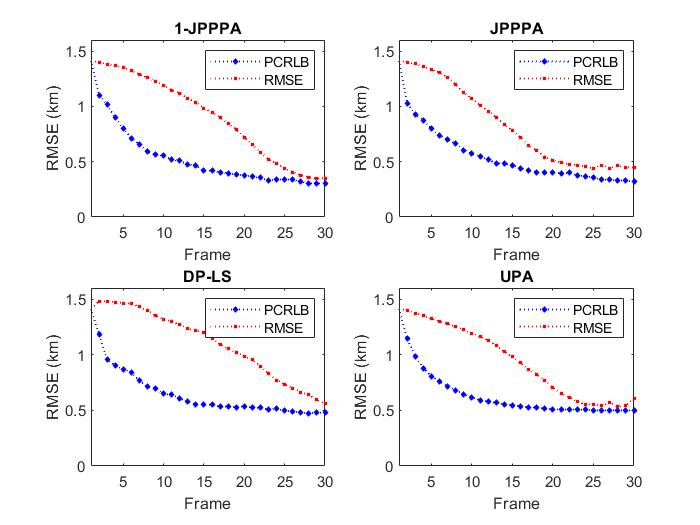
\includegraphics[scale=0.72]{RMSE.jpg}
	\caption{Comparison of position MSE of Target 1 between different resource management strategies}
	\label{fig:RMSE}
\end{figure*}

%Iyemeh: Since the plots all have a common vertical and horizontal axes, i would suggest merging the curves and making it bigger so that the reader can appreciate the difference. 

\begin{table*}
	
	\centering
%	\fontsize{6.5}{8}\selectfont
	
		\caption{Comparison of Position RMSE between Different Resource Management Strategies}
		\label{tab:performance_comparison}
		\begin{tabular}{ccccccccccc}
			\toprule
			\multirow{2}{*}{Strategy}&
			\multicolumn{5}{c}{PCRLB (m)}&\multicolumn{5}{c}{ RMSE (m)}\cr
			\cmidrule(lr){2-6} \cmidrule(lr){7-11}
			&Target 1&Target 2&Target 3&Target 4&Target 5&Target 1&Target 2&Target 3&Target 4&Target 5\cr
			\midrule
			1-JPPPA&305.4&461.6&489.1&317.2&563.2&354.2&546.1&538.6&436.2&912.6\cr
			JPPPA&318.1&471.2&478.3&388.6&621.1&446.7&538.1&472.2&489.4&870.9\cr
			DP-LS&481.5&492.7&488.7&547.0&794.7&559.3&876.6&666.9&797.7&1248.6\cr
			UPA&497.9&492.3&477.7&553.8&822.6&604.0&598.4&592.1&654.8&1472.3\cr
			\bottomrule
		\end{tabular}
	\label{tab:RMSE}
\end{table*}

\subsection{Evaluation of the Custom Pre-selection Operator}
Simulation I and II %Iyemeh: This is not clear. What are they? If they are names for some specific analyses carried out, they have not been used in this paper before now. A way to go about it is to state what Simulation I and II are before using them. 
are identical to the previous simulations on 1-JPPPA and JPPPA, respectively. In the population generated by the pre-selection operator, 10\% of individuals are offsprings of the elite and another random individual; 10\% of the individuals are mutated from the elite. The reader is reminded that the mutation in the pre-selection operator is different from the normal mutation. In simulation III, the pre-selection operator is not used, and the initial population at each time step is generated randomly. All simulations are conducted using MATLAB R2019a on a laptop with a Core\texttrademark\ i5 2.6 GHz CPU and 8 GB RAM.

\begin{figure}
	\centering
	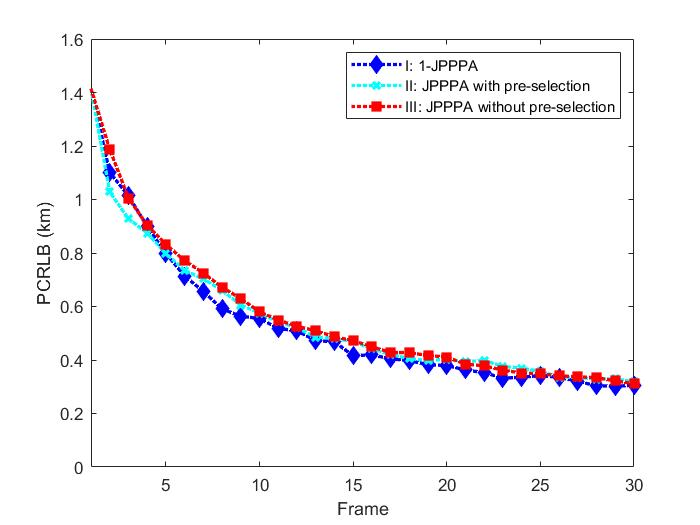
\includegraphics[scale=0.36]{Pre Selection.jpg}
	\caption{Comparison between algorithms with and without the pre-selection operator}
	\label{fig:Pre-selection}
\end{figure}


 \begin{table}
	\centering
	\caption{Comparison of Speed between Different Algorithms}
	\begin{tabular}{cccc}
		\toprule
		Simulation & Generations & Time per Frame (s) & Total Time (s)\\ 
		\midrule
		I & 24.28 & 1.451 & 60.85\\ 
		II & 15.74 & 2.732 & 95.64\\ 
		III & 22.19 & 3.827 & 131.40\\ 
		\bottomrule
	\end{tabular}
	\label{tab:Pre-selection}
\end{table}



The true PCRLB values calculated with the optimization results that are obtained by three algorithms are presented in Fig. \ref{fig:Pre-selection}. The three algorithms have similar performance. Table \ref{tab:Pre-selection} demonstrates the speed of three algorithms. The average number of generations when the GA terminates is recorded in column 2. Column 3 and 4 give the average processing time of one frame and of the whole surveillance period respectively. Note that the particle filter requires certain amount of time due to large number of particles.

It can be seen in Table \ref{tab:Pre-selection} that Simulation II takes less time while it achieves nearly the same result as Simulation III in Fig. \ref{fig:Pre-selection}, which verifies the efficiency of the proposed pre-selection operator under the RHC framework. The population spends less generations evolving due to the existence of the prior information. From Table \ref{tab:Pre-selection},  it can be seen that Simulation II takes about one second less to make decisions at each epoch compared to Simulation III, which is vital in practice. Moreover, in a radar system that adopts RHC, the receivers will get commands on speed and heading angle in future steps, which makes the system less vulnerable to emergency situations such as communication failure. %Iyemeh: This needs to be related to the results being discussed. At the moment, we just moved from the simulation comparison to RHC. It seems disjointed. Rephrase to make the paragraph read smoothly. 

Note that the average generation in Simulation III is less than Simulation I, which means the solver terminiates in Simulation I when the maximum generation is reached while in Simulation III when no improvement can be found in the past 5 generations. It can be inferred that the solver in Simulation III is stuck in a local minimum and the crossover and mutation operators cannot get it out of the local minimum. This is consistent with our previous statement that it is more difficult to find a best combination of genes when chromosomes become longer. Further research can be done on the modification of crossover and mutation operators to reduce the probability of the solver being stuck in local minimum. 

GA is characterized as an \emph{unguided} heuristic algorithm, which is both an advantage and a disadvantange. GA is advantageous because the user does not need to know how the population evolves, only discarding unfitted individuals is required. On the other hand, however, it also causes inefficiency when the algorithm starts to converge since improvement is generally achieved by randomness. 

With the pre-selection operator, a small proportion of individuals are more likely to be generated around the prior information, and the solver is more probable to search for candidates in that area. As previously stated in Section IV, the pre-selection operator is similar to giving more weight to an individual in a particle swarm optimization (PSO), i.e., advantages of PSO are incorporated into the solver through the custom pre-selection operator. The challenge with population generation  %Iyemeh: I have modified this sentence for clarity. Rephrase if it does not convey your point.   
under the RHC framwork is that there might exist useful information to provide guidance for the evolution of the population. Modifying the algorithm by making use of such information will improve the peformance.

\subsection{Factors that Affect JPPPA Results}
To demonstrate other factors that affect the JPPPA result, another set of simulations is presented in this subsection. The simulations are conducted to reveal the effect of target RCS and bistatic ranges on the JPPPA optimization results. To enhance the effect of these factors, the simulation case is simplified by removing target 5, receiver 4 and receiver 5.%Iyemeh: include the figure to which the reader should note where the traget 5, receiver 4 and 5 are.  

Two different RCS models $\mathbf{H_1}$ and $\mathbf{H_2}$ are provided. In $\mathbf{H_1}$, all targets' RCS are modeled by the Swerling I model, i.e., the RCS is a random number that satisfies a chi-squared distribution with two degrees of freedom but remains constant over the measurement scan. In $\mathbf{H_2}$, the RCS model of targets 3, and 4 remain unchanged, while targets 1 and 2 are assumed to have larger RCS. Fig. \ref{fig:RCS} shows the RCS of all targets in this scenario.

There are also two different transmitter locations, ${\mathbf{Tx_1}}: (0,0)$ and $\mathbf{Tx_2}:(40,10)$ available. In case $\mathbf{Tx_1}$, all targets have similar overall bistatic ranges with respect to all bistatic pairs while in $\mathbf{Tx_2}$, with the transmitter located in the first quadrant, some targets will have significantly increased bistatic ranges. %Iyemeh: This can be better introduced. The figure needs to be discussed before switching discussions to different transmitter locations. 

\begin{figure}
	\centering
	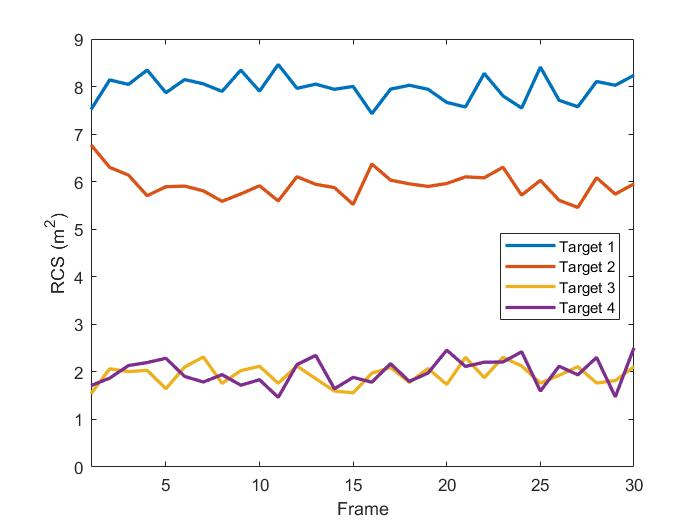
\includegraphics[scale=0.36]{RCS.jpg}
	\caption{RCS of different targets in scenario $\mathbf{H_2}$}
	\label{fig:RCS}
\end{figure}
%Iyemeh: This figure was not discussed in the text. Extract more information from the figure and discuss, otherwise it only consumes space in the paper. 

Simulations are conducted on three different scenarios:

(1) case 1: $\mathbf{H_1}$ and $\mathbf{Tx_1}$;

(2) case 2: $\mathbf{H_2}$ and $\mathbf{Tx_1}$;

(3) case 3: $\mathbf{H_1}$ and $\mathbf{Tx_2}$.

The power allocation results are presented from Fig. \ref{fig:Power 1} to Fig. \ref{fig:Power 3}. %Iyemeh: Combine plots into one figure. You will then have 9a, 9b, and 9c. Keeping them together will help readers appreciate the discussion. 
 It can be intuitively seen that in case 1, targets 1 and 2 are allocated with more power while in case 2, the overall power scheme between targets 1 and 2 is more even and is less than that in case 1. %Iyemeh:I have modified the sentence. Rephrase if it is incorrect. 
  The power radiation values at time step 30 are give in Table \ref{tab:Power between RCS}. It can be concluded that the transmitter tends to illuminate the target with relatively low RCS.

\begin{figure}
	\centering
	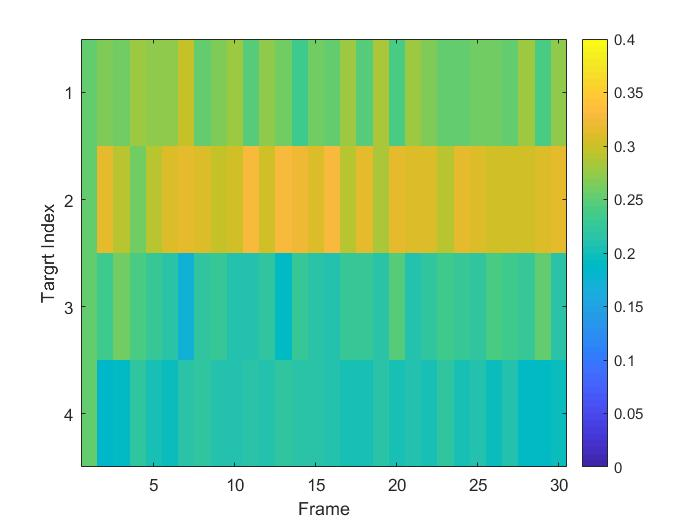
\includegraphics[scale=0.36]{Power1.jpg}
	\caption{Power allocation result of case 1}
	\label{fig:Power 1}
\end{figure}

\begin{figure}
	\centering
	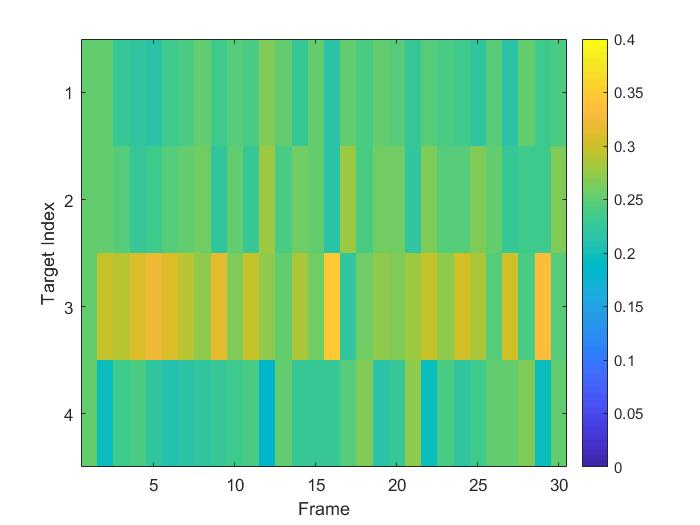
\includegraphics[scale=0.36]{Power2.jpg}
	\caption{Power allocation result of case 2}
	\label{fig:Power 2}
\end{figure}

\begin{figure}
	\centering
	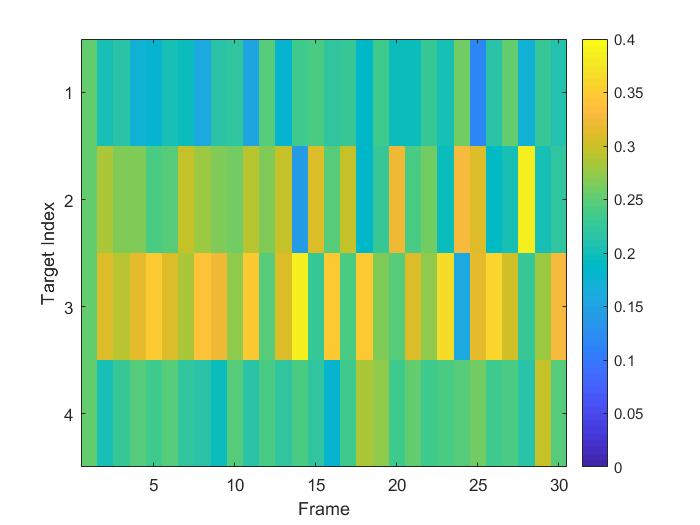
\includegraphics[scale=0.36]{Power3.jpg}
	\caption{Power allocation result of case 3}
	\label{fig:Power 3}
\end{figure}


%\emph{Remark:} If the target RCS can be modeled precisely and can be measured by the radar, it is more favorable to augment the target state and track the RCS. With the RCS become predictive, the solver will 

From Fig. \ref{fig:Power 3}, we can easily see that after the transmitter is moved from the origin to (40,10), there is a significant increase in the power radiation that is allocated to track target 3, which is located in the third quadrant % Iyemeh:Fig. 4 is the only plot that shows any form of transmitter/receiver orientation and it is all the way back in page 22. I would suggest a modified version is brought closer to the point where the cases were described. This will help the reader follow discussions with regards to the change in orientation. 
 and thus has the largest overall bistatic ranges. Meanwhile, target 1 that is located in the first quadrant, being closer to the transmitter, is now assigned with less power. Table \ref{tab:Power between Range} gives the power allocation result and the bistatic ranges with respect to three receivers at time step 30. Although the exact mathematical relationship between the bistatic range and the allocated power is hard to determine with the simulation results presented since the system is configured with more than one receiver, it can be roughly concluded that the transmitter tends to assign more power to targets with large bistatic ranges under the objective of optimizing overall tracking performance.

\begin{table*}
	
	\centering
	
	\caption{Comparison of the Power Allocated in Cases 1 and 2}
	%Iyemeh: Rephrase needed. Suggestion: Comparison of the Power Allocated in Case 1 and 2
	\label{tab:performance_comparison}
	\begin{tabular}{ccccc}
		\toprule
		\multirow{2}{*}{Target Index}&
		\multicolumn{2}{c}{Case 1}&\multicolumn{2}{c}{Case 2}\cr
		\cmidrule(lr){2-3} \cmidrule(lr){4-5}
		&RCS (m$^2$)&Power Allocated&RCS (m$^2$)&Power Allocated\cr
		\midrule
		1 & 2.11 & 0.2641 & 8.71 & 0.2438\cr
		2 & 1.58 & 0.3045 & 7.74 & 0.2652\cr
		3 & 1.71 & 0.2280 & 2.06 & 0.2587\cr
		4 & 2.19  & 0.2034 & 1.60 & 0.2323\cr
		\bottomrule
	\end{tabular}
	\label{tab:Power between RCS}
\end{table*}

\begin{table*}
	
	\centering
	
	\caption{Power Allocation Result and Bistatic Range}
	\label{tab:performance_comparison}
	\begin{tabular}{ccccc}
		\toprule
		\multirow{2}{*}{Target Index}&
		\multicolumn{3}{c}{Bistatic Range (km)}&\multirow{2}{*}{Power Allocated}\cr
		\cmidrule(lr){2-4}
		&W.r.t Receiver 1&W.r.t Receiver 2&W.r.t Receiver 3\cr
		\midrule
		1 & 98.34 & 138.32 & 145.89 & 0.2641 \cr
		2 & 131.35 & 91.52 & 131.16 & 0.3045\cr
		3 & 141.40 & 111.31 & 97.33 & 0.2280 \cr
		4 & 99.19 & 122.02 & 87.91 & 0.2034 \cr
		\bottomrule
	\end{tabular}
	\label{tab:Power between Range}
\end{table*}

\emph{Remark 6:} The transmitter will allocate more power to illuminate targets with low SNR (small RCS, large bistatic range, etc.). This may not be a wise resource management strategy if these factors that affect the optimization result have a significant difference among targets. For example, if target 1 and target 2 have a RCS of 1 unit and 100 units respectivley, and other parameters are identical, the transmitter would allocate 100 units of power to target 1 and 1 unit to target 2, which might waste limited resources on targets that are already hard enough to track.% Iyemeh: Logically, it makes sense to channel power to targets that are far away as you will need to overcome high pathloss in order to reach them. If this is not done, the system will only be able to track tragets within a small range which will negate the use of radars. 
 In a multistatic radar system with more than 1 transmitters, a clever approach for a transmitter is to discard such targets and let other transmitters with better bistatic geometries illuminate them. These problems are addressed in the literature as beam selection, base station selection, etc. %Iyemeh: Include citation for these literatures. 
  Future research will investigate multistatic radar systems with multiple transmitters. 


\section{Conclusion}

In this paper, a JPPPA strategy for multitarget tracking in a multistatic radar system was proposed. The radar adopts a multibeam mode that tracks multiple targets simultaneously, and the receivers are mounted on UAVs whose trajectories are to be optimized for better tracking peformance. The basis of the proposed strategy is the cooperative receding horizon control of both power allocation pattern and UAV trajectories based on PCRLB. The formulated problem is a three-variable nonconvex problem, and a modified GA with a custom pre-selection operator was proposed to solve the problem. It was shown that our method does not depend on the convexity of the objective function, and can be applied to more complicated scenarios. Numerical simulations were performed to demonstrate the effectiveness of the proposed JPPPA strategy and its advantage over methods that consider path planning and power allocation respectively. 

This work can be extended by considering the following issues. First, the JPPPA problem can be tackled jointly with beamforming, beam selection and radar mode selection in more complex radar configurations. Second, the number of target is assumed to be known and fixed in this work. Future research will explore scenarios where the number of targets are unknown by applying the optimal resource management strategies to tracking problems based on random finite set (RFS).

\bibliographystyle{IEEEtran}
\bibliography{reference}
\end{document}